\documentclass[tikz,border=0pt]{standalone}
\usepackage{iftex}
\ifLuaTeX
\usepackage{fontspec}
\setsansfont{DejaVu Sans}
\else
\usepackage[T1]{fontenc}
\usepackage[utf8]{inputenc}
\usepackage{lmodern}
\fi
\usepackage{amsmath}
\usetikzlibrary{arrows.meta}
\renewcommand{\familydefault}{\sfdefault}
\definecolor{adbg}{HTML}{101827}
\definecolor{adfg}{HTML}{F1F5F9}
\definecolor{admuted}{HTML}{B5C4D9}
\definecolor{adline}{HTML}{A9BDD8}
\definecolor{adgroup}{HTML}{172236}
\definecolor{adborder}{HTML}{435470}
\definecolor{adinput}{HTML}{93C5FD}
\definecolor{adinputfill}{HTML}{202E44}
\definecolor{adcompute}{HTML}{5EEAD4}
\definecolor{adcomputefill}{HTML}{202E44}
\definecolor{admodel}{HTML}{C4B5FD}
\definecolor{admodelfill}{HTML}{202E44}
\definecolor{admemory}{HTML}{7DD3FC}
\definecolor{admemoryfill}{HTML}{202E44}
\definecolor{adtool}{HTML}{FCD34D}
\definecolor{adtoolfill}{HTML}{202E44}
\definecolor{adcontrol}{HTML}{CBD5E1}
\definecolor{adcontrolfill}{HTML}{202E44}
\definecolor{adoutput}{HTML}{6EE7B7}
\definecolor{adoutputfill}{HTML}{202E44}
\definecolor{adneutral}{HTML}{CBD5E1}
\definecolor{adneutralfill}{HTML}{202E44}
\begin{document}
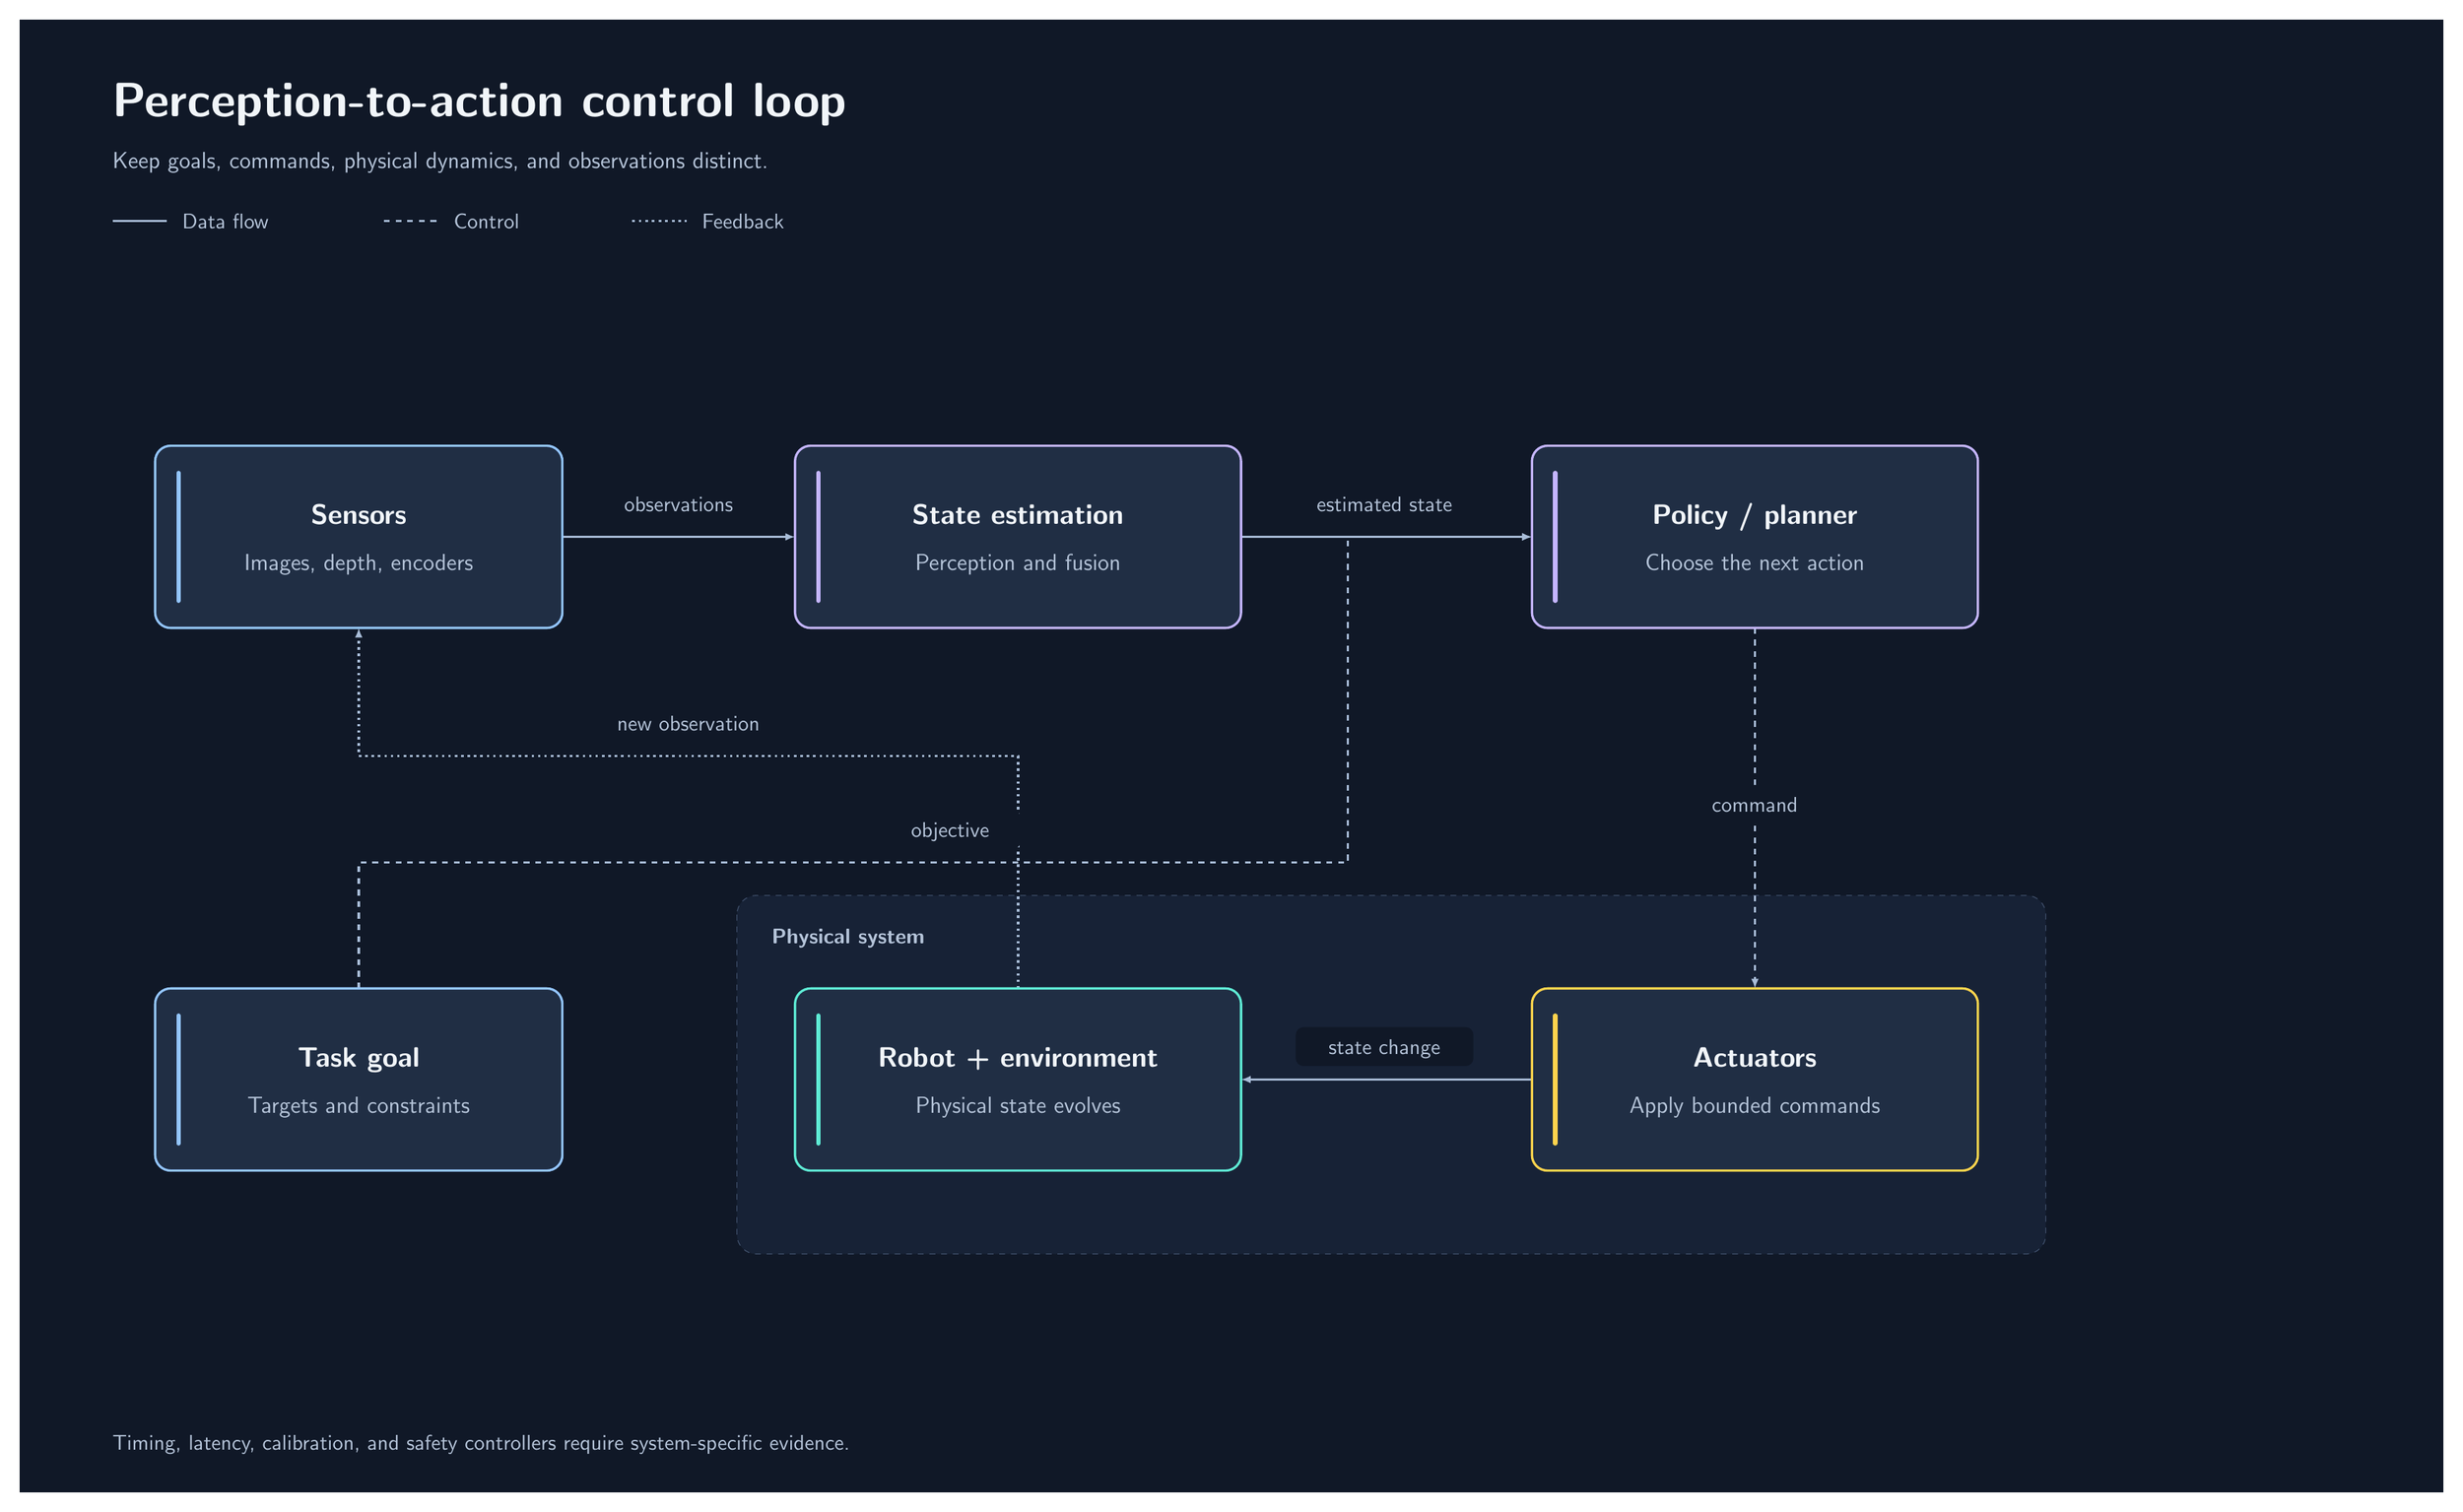
\begin{tikzpicture}[x=1pt,y=-1pt,inner sep=0pt,outer sep=0pt]
\path[use as bounding box] (0,0) rectangle (1250,760);
\fill[adbg] (0,0) rectangle (1250,760);
\node[anchor=base west,text=adfg,font={\sffamily\fontsize{29}{34.8}\selectfont\bfseries}] at (48,50) {Perception-to-action control loop};
\node[anchor=base west,text=admuted,font={\sffamily\fontsize{13}{15.6}\selectfont}] at (48,77) {Keep goals, commands, physical dynamics, and observations distinct.};
\draw[adline,line width=1.4pt] (48,104) -- (76,104);
\node[anchor=base west,text=admuted,font={\sffamily\fontsize{10.5}{12.6}\selectfont}] at (84,108) {Data flow};
\draw[adline,line width=1.4pt,dashed] (188,104) -- (216,104);
\node[anchor=base west,text=admuted,font={\sffamily\fontsize{10.5}{12.6}\selectfont}] at (224,108) {Control};
\draw[adline,line width=1.4pt,dotted] (316,104) -- (344,104);
\node[anchor=base west,text=admuted,font={\sffamily\fontsize{10.5}{12.6}\selectfont}] at (352,108) {Feedback};
\draw[fill=adgroup,draw=adborder,dashed,rounded corners=10pt] (370,452) rectangle (1045,637);
\node[anchor=base west,text=admuted,font={\sffamily\fontsize{11}{13.2}\selectfont\bfseries}] at (388,477) {Physical system};
\draw[adline,line width=1.3pt,-{Latex[length=5pt,width=4pt]},line join=round] (280,267) -- (340,267) -- (400,267);
\draw[adline,line width=1.3pt,-{Latex[length=5pt,width=4pt]},line join=round] (630,267) -- (705,267) -- (780,267);
\draw[adline,line width=1.3pt,-{Latex[length=5pt,width=4pt]},line join=round,dashed] (895,314) -- (895,407) -- (895,500);
\draw[adline,line width=1.3pt,-{Latex[length=5pt,width=4pt]},line join=round] (780,547) -- (705,547) -- (630,547);
\draw[adline,line width=1.3pt,-{Latex[length=5pt,width=4pt]},line join=round,dotted] (515,500) -- (515,380) -- (175,380) -- (175,314);
\draw[adline,line width=1.3pt,-{Latex[length=5pt,width=4pt]},line join=round,dashed] (175,500) -- (175,435) -- (685,435) -- (685,267) -- (780,267);
\draw[draw=adinput,fill=adinputfill,line width=1.2pt,rounded corners=8pt] (70,220) rectangle (280,314);
\draw[adinput,line width=2.2pt,line cap=round] (82,234) -- (82,300);
\node[anchor=base,text=adfg,font={\sffamily\fontsize{15}{18.0}\selectfont\bfseries}] at (175,260.5) {Sensors};
\node[anchor=base,text=admuted,font={\sffamily\fontsize{11.5}{13.799999999999999}\selectfont}] at (175,284.5) {Images, depth, encoders};
\draw[draw=admodel,fill=admodelfill,line width=1.2pt,rounded corners=8pt] (400,220) rectangle (630,314);
\draw[admodel,line width=2.2pt,line cap=round] (412,234) -- (412,300);
\node[anchor=base,text=adfg,font={\sffamily\fontsize{15}{18.0}\selectfont\bfseries}] at (515,260.5) {State estimation};
\node[anchor=base,text=admuted,font={\sffamily\fontsize{11.5}{13.799999999999999}\selectfont}] at (515,284.5) {Perception and fusion};
\draw[draw=admodel,fill=admodelfill,line width=1.2pt,rounded corners=8pt] (780,220) rectangle (1010,314);
\draw[admodel,line width=2.2pt,line cap=round] (792,234) -- (792,300);
\node[anchor=base,text=adfg,font={\sffamily\fontsize{15}{18.0}\selectfont\bfseries}] at (895,260.5) {Policy / planner};
\node[anchor=base,text=admuted,font={\sffamily\fontsize{11.5}{13.799999999999999}\selectfont}] at (895,284.5) {Choose the next action};
\draw[draw=adtool,fill=adtoolfill,line width=1.2pt,rounded corners=8pt] (780,500) rectangle (1010,594);
\draw[adtool,line width=2.2pt,line cap=round] (792,514) -- (792,580);
\node[anchor=base,text=adfg,font={\sffamily\fontsize{15}{18.0}\selectfont\bfseries}] at (895,540.5) {Actuators};
\node[anchor=base,text=admuted,font={\sffamily\fontsize{11.5}{13.799999999999999}\selectfont}] at (895,564.5) {Apply bounded commands};
\draw[draw=adcompute,fill=adcomputefill,line width=1.2pt,rounded corners=8pt] (400,500) rectangle (630,594);
\draw[adcompute,line width=2.2pt,line cap=round] (412,514) -- (412,580);
\node[anchor=base,text=adfg,font={\sffamily\fontsize{15}{18.0}\selectfont\bfseries}] at (515,540.5) {Robot + environment};
\node[anchor=base,text=admuted,font={\sffamily\fontsize{11.5}{13.799999999999999}\selectfont}] at (515,564.5) {Physical state evolves};
\draw[draw=adinput,fill=adinputfill,line width=1.2pt,rounded corners=8pt] (70,500) rectangle (280,594);
\draw[adinput,line width=2.2pt,line cap=round] (82,514) -- (82,580);
\node[anchor=base,text=adfg,font={\sffamily\fontsize{15}{18.0}\selectfont\bfseries}] at (175,540.5) {Task goal};
\node[anchor=base,text=admuted,font={\sffamily\fontsize{11.5}{13.799999999999999}\selectfont}] at (175,564.5) {Targets and constraints};
\fill[adbg,rounded corners=4pt] (294.2,240) rectangle (385.8,260);
\node[anchor=base,text=admuted,font={\sffamily\fontsize{11}{13.2}\selectfont}] at (340,254) {observations};
\fill[adbg,rounded corners=4pt] (648.75,240) rectangle (759.25,260);
\node[anchor=base,text=admuted,font={\sffamily\fontsize{11}{13.2}\selectfont}] at (704,254) {estimated state};
\fill[adbg,rounded corners=4pt] (864.95,395) rectangle (925.05,415);
\node[anchor=base,text=admuted,font={\sffamily\fontsize{11}{13.2}\selectfont}] at (895,409) {command};
\fill[adbg,rounded corners=4pt] (658.2,520) rectangle (749.8,540);
\node[anchor=base,text=admuted,font={\sffamily\fontsize{11}{13.2}\selectfont}] at (704,534) {state change};
\fill[adbg,rounded corners=4pt] (289.75,353) rectangle (400.25,373);
\node[anchor=base,text=admuted,font={\sffamily\fontsize{11}{13.2}\selectfont}] at (345,367) {new observation};
\fill[adbg,rounded corners=4pt] (443.65,408) rectangle (516.35,428);
\node[anchor=base,text=admuted,font={\sffamily\fontsize{11}{13.2}\selectfont}] at (480,422) {objective};
\node[anchor=base west,text=admuted,font={\sffamily\fontsize{11}{13.2}\selectfont}] at (48,738) {Timing, latency, calibration, and safety controllers require system-specific evidence.};
\end{tikzpicture}
\end{document}
